% -----------------------------------------------
% Template for ISMIR Papers
% 2017 version, based on previous ISMIR templates

% Requirements :
% * 6+n page length maximum
% * 4MB maximum file size
% * Copyright note must appear in the bottom left corner of first page
% * Clearer statement about citing own work in anonymized submission
% (see conference website for additional details)
% -----------------------------------------------

\documentclass{article}
\usepackage{ismir,amsmath,cite,url}
\usepackage{graphicx}
\usepackage{color}
\usepackage{microtype}
\usepackage{units}
\usepackage{graphicx}
\usepackage{multirow}
\usepackage{paralist}

% Title.
% ------
\title{Automatic assessment of percussive instrument performances with sparse coding}

% Note: Please do NOT use \thanks or a \footnote in any of the author markup

% Single address
% To use with only one author or several with the same address
% ---------------
%\oneauthor
% {Names should be omitted for double-blind reviewing}
% {Affiliations should be omitted for double-blind reviewing}

%\oneauthor
%{Chih-Wei Wu, Alexander Lerch}
%{Georgia Institute of Technology, Center for Music Technology \\ \tt \{cwu307, alexander.lerch\}@gatech.edu}
 
% Two addresses
% --------------
%\twoauthors
%  {First author} {School \\ Department}
%  {Second author} {Company \\ Address}

%% To make customize author list in Creative Common license, uncomment and customize the next line
%  \def\authorname{First Author, Second Author}


% Three addresses
% --------------
\threeauthors
  {First Author} {Affiliation1 \\ {\tt author1@ismir.edu}}
  {Second Author} {\bf Retain these fake authors in\\\bf submission to preserve the formatting}
  {Third Author} {Affiliation3 \\ {\tt author3@ismir.edu}}

%% To make customize author list in Creative Common license, uncomment and customize the next line
%  \def\authorname{First Author, Second Author, Third Author}

% Four or more addresses
% OR alternative format for large number of co-authors
% ------------
%\multauthor
%{First author$^1$ \hspace{1cm} Second author$^1$ \hspace{1cm} Third author$^2$} { \bfseries{Fourth author$^3$ \hspace{1cm} Fifth author$^2$ \hspace{1cm} Sixth author$^1$}\\
%  $^1$ Department of Computer Science, University , Country\\
%$^2$ International Laboratories, City, Country\\
%$^3$  Company, Address\\
%{\tt\small CorrespondenceAuthor@ismir.edu, PossibleOtherAuthor@ismir.edu}
%}
%\def\authorname{First author, Second author, Third author, Fourth author, Fifth author, Sixth author}


\sloppy % please retain sloppy command for improved formatting

\begin{document}

%
\maketitle
%
\begin{abstract}
The automatic assessment of (student) music performance involves the characterization of the audio recordings and the modeling of human judgments. To build a computational model that provides a reliable assessment, the system must take into account various aspects of a performance including technical correctness and aesthetic standards. While some progress has been made in recent years, the search for the most effective feature representation remains open-ended. In this study, we explore the possibility of using learned features from sparse coding. Specifically, we investigate the effectiveness of different combinations of three sets of features, namely a baseline set, a set of designed features, and a learned feature set. In addition, we compare the effectiveness of sparse coding based on different input representations. The proposed feature sets are evaluated in regression tasks on a dataset of annotated recordings of students playing snare exercises. The results imply the general viability of feature learning in the context of automatic assessment of snare drum performances.   
\end{abstract}
%
\section{Introduction}
Music performance is a sequence of actions that integrates both cognitive and motor skills. Starting from the musical ideas, this process of converting thoughts into movements, as pointed out by Palmer \cite{Palmer1997}, is among the most skill intensive actions produced by human beings. To cultivate these skills, the qualitative assessment from the peers and teachers is an essential pedagogical component in music education. A systematic assessment that facilitates improvements usually requires a careful examination of different aspects of a performance, such as technical correctness and aesthetics. This task, however, is extremely difficult due to its subjective nature. As a result, human raters tend to exhibit a large variance in terms of their severity, rating scale, and the interpretation of rating categories \cite{Wesolowski2016}; the bias of the raters and the ill-defined categories, as suggested by Thompson and Williamon \cite{Thompson2003}, could adversely impact the discriminability and the fairness of assessment. Therefore, a computational approach that provides consistent and repeatable feedback might offer a potential solution to this issue and enhance the learning experience of the students. 

With the recent advances in the field of Music Information Retrieval (MIR), such as music transcription \cite{Benetos2013} and source separation \cite{Huang2014}, the realization of intelligent music systems with reliable functionalities become pausible, opening up new possibilities for music education \cite{Dittmar2012}. Commercial software such as SmartMusic\footnote{http://www.smartmusic.com Last access: 2017/04/26} and Yousician\footnote{http://yousician.com Last access: 2017/04/26} both showcase of how automatic assessment tools could support the music learning process with more flexible practice sessions. These efforts, while providing basic solutions to the users, still fell short in characterizing the abstract aspect of a performance such as musicality. This limitation usually originates from the design of the audio features. In MIR, a set of well-established features has proven to be successful in applications such as music genre classification \cite{Tzanetakis2002}, however, the direct adoption of these features without further adjustments often lead to sub-optimal performances, and the fine-tuning of the features could be difficult and time-consuming.

In this paper, we explore the possibility of applying unsupervised feature learning in the context of music performance assessment. In particular, we compare the effectiveness of the baseline features, designed features, and leanred features in assessing students' snare drum performances during the All-state auditions. The contributions this paper include:
\begin{inparaenum}[(i)]
	\item   new insights into the viability of applying feature learning to the problem of automatic music performance assessment, 
    \item   a new input representation that characterizes percussive instrument performances for feature learning purposes, and 
    \item   the demonstration of potential improvements in predicting judges' ratings using the proposed method.
\end{inparaenum} 
The general goal of this paper is to efficiently find the optimal features for characterizing percussive instrument performances. The rest of the paper is structured as follows: Sect.~\ref{sec:relatedwork} presents the related work in automatic music performance assessment and feature learning. In Sect.~\ref{sec:method}, we introduce our proposed method. The experiment setup and results are described in Sect.~\ref{sec:experiments}. Finally, the conclusion and future directions are presented in Sect.~\ref{sec:conclusion}.

\section{Related Work}\label{sec:relatedwork}
% MPA with designed features
Music Perofrmance Analysis (MPA) is a research field that concerns the study of the acoustic rendition of music \cite{Lerch2012}. To automate this process, a system must handle the extraction and interpretation of the important parameters of music performances. In the early research, most of the analysis was performed on symbolic data extracted from external sensors or MIDI devices. Recently, the focus has gradually shifted to the analysis of audio recordings. The basic approach to this problem usually involves the careful design of audio features that are capable of extracting the most relevant information in different contexts. For instance, Nakano presented an automatic system that evaluates the singing skill of the users \cite{Nakano2006a}. By characterizing the performances through pitch interval accuracy and vibrato features, the system has shown to be able to classify the performance into two classes (good or poor) with high accuracy. Isabel et al.~ present a system that identifies the violin techniques, such as pizzicato and vibrato, using both temporal and spectral features\cite{Barbancho2009}. With a hierachical decision flow, the system achieves high accuracy in differentiating 7 techniques. Abe{\ss}er et al.\ propose a system that automatically assesses the quality of vocal and instrumental performances of 9th and 10th graders \cite{Abeßer2013}. Features that measure the pitch, intonation and rhythmic correctness are created to quantify the students' performances. The evaluation results show that the system is able to predict four different performance qualities with ocassional confusions between the adjacent classes. In a system that identifies the common mistakes by the flute beginners, Han and Lee propose to use dedicated features for detecting events such as poor blowing and misfingering\cite{Han2014}. More recently, Wu et al.~ propose to assess students' instrumental performances using a set of features derived from pitch, amplitude, and inter-onset interval histograms\cite{Wu2016}. The evaluation results show reasonable correlation between the model predictions and the judges' ratings. 

\begin{figure}
\centering
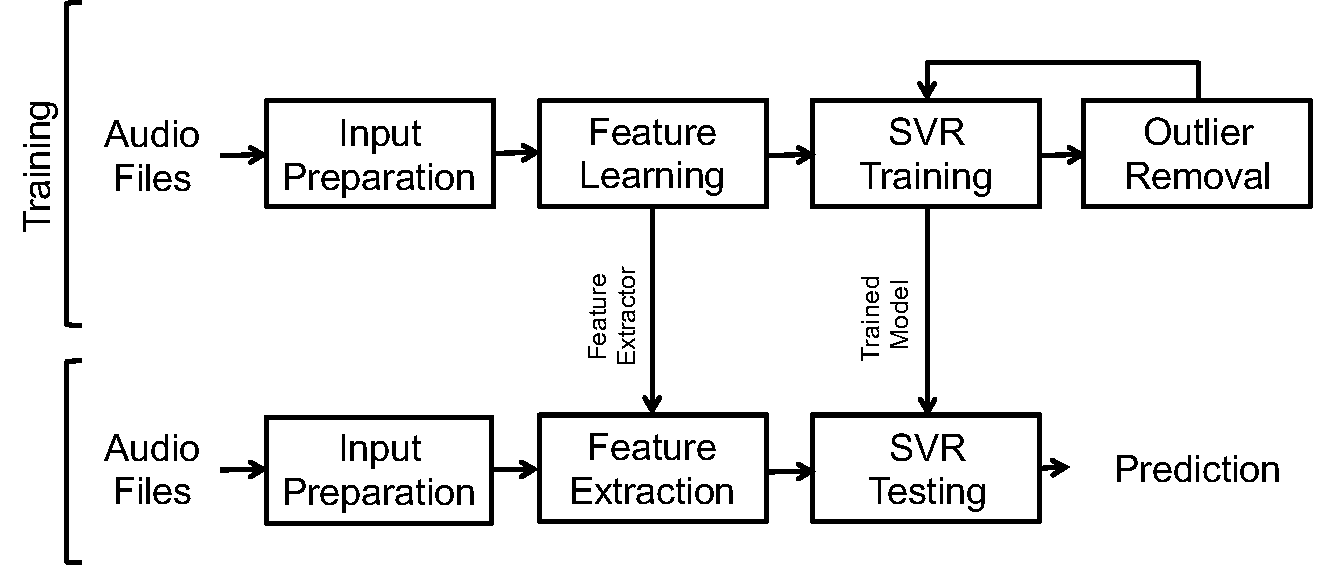
\includegraphics[width = 8 cm]{./figs/flowchart.pdf}
\caption{The flowchart of the proposed method.}
\label{fig:flowchart}
\end{figure}

All of the above mentioned systems use designed features in the analysis pipeline. This approach, while translating the music domain knowledge into the machine operations, does not take advantage of the internal structure of the data. Feature learning, on the opposite, allows the algorithm to find the most fitting features based on the given input representations. Several feature learning methods have been found successful in music related applications. For example, Lee et al.~ propose to apply Convolutional Deep Belief Networks (CDBNs) on magnitude spectrogram to learn features \cite{Lee2009a}; the evalution results show that the learned features outperform the convetional audio features on a music genre classification task. Following the similar direction, Hamel and Eck demonstrate that a Deep Belief Network (DBN) is able to derive features that achieve state-of-the-art performance in genre classification \cite{Hamel2010}. With the same task, Henaff et al.~ apply Sparse Coding (SC) algorithm on the log spectrogram and use the learned features to train a SVM classifier. The evaluation results also indicate the effectiveness of the learned features in the context of genre classification. Nam et al.~ further introduce a pre-processing pipeline that improves the SC feature learning \cite{Nam2012}; the evaluation results on a music tagging dataset compare favorably against the commonly used audio features.   

\section{Method}\label{sec:method}
\subsection{System Overview}
In this paper, the proposed system comprises both training and testing phase. As shown in Fig.~\ref{fig:flowchart}, the training phase starts by processing each audio recording of student performance into the input representation; the input representations in the training data are collected and passed onto the feature learning block. In the feature learning step, the feature extractor is dervied by solving the optimization problem across entire dataset, and the corresponding feature vector for each recording is calculated. Finally, the features are used to train a regression model that minimizes the loss between the model prediction and the ground truth (judges' ratings) for each recording, along with an outlier removal step to refine the model. 

In the testing phase, a similar procedure is taken for each recording to prepare the input representation and extract features using the derived feature extractor. The resulting feature vector is used to predict the judges' ratings with the pre-trained regression model. In the following sections, more details of each major building blocks are presented. 

\subsection{Input Preparation}\label{subsec:input}
% talk about two different inpu representations I tried
% STFT & IOI hist
In the input preparation step, audio recordings in mp3 format are first down-mixed to mono and resampled to a sampling rate = \unit[22.05]{kHz}. All the files are normalized to a numerical range between -1 and 1. Next, two different matrix representations are computed, namely the Short-Time Fourier Transform (STFT) and local histogram matrix. 

\subsubsection{STFT}\label{subsec:stft}
For STFT, it is computed using a block of 512 samples with 50 \% overlapping blocks; a Hann window is applied to each block. In our experiments, only the magnitude spectrogram is used, and the phase information is discarded. The resulting magnitude spectrogram $M_{stft}$ is a $m \times n$ matrix, in which $m = 257$ and $n = $ the number of blocks. This input representation has been used extensively in SC related literature as a baseline input \cite{Su2014Guitar, Su2014Violin}. 

\subsubsection{Local Histogram Matrix}
The Local Histogram Matrix (LHM) is our proposed input representation to the feature learner that aims to capture the essence of the percussive instrument performances. The extraction process of the local histogram matrix is shown in Fig.~\ref{fig:hist_mat}. To begin with, the input time-domain audio signal is partitioned into 10-second non-overlapping local segments. This number is chosen in order to capture higher level structure such as music paragraphs. Within each segment, $\mathbf{v}_{ioi}$, $\mathbf{v}_{amp}$, and $\mathbf{v}_{mfcc}$ are calculated locally, in which $\mathbf{v}_{ioi}$ is the Inter-Onset-Interval (IOI) histogram vector, $\mathbf{v}_{amp}$ is the amplitude histogram vector, and $\mathbf{v}_{mfcc}$ is the averaged MFCCs vector. Concatenating these vectors will result in local histogram matrix $M_{lhm}$ that represents each individual recording. The definitions of these vectors are explained as follows:

\begin{itemize}
\item[(i)] \textbf{IOI histogram vector ($\mathbf{v}_{ioi}$)}: first, the onset times within the local segment are estimated using a standard spectral flux novelty function and an adaptive median threshold for peak picking, resulting in a vector $onset(i)$ in which $i$ is the onset index; the implementation follows the descriptions in \cite{Lerch2012}. The IOI sequence is calculated by $IOI = diff(onset(i))$, followed by a non-linear transformation $IOI_{ln} = ln(IOI)$. Next, the $V_{ioi}$ is computed by estimating the histogram from the $IOI_{ln}$ with a pre-defined range and resolution, which are both determined through data observation in our preliminary experiments. Finally, the $\mathbf{v}_{ioi}$ is normalized by dividing the total number of onsets in the entire recording. The resulting $\mathbf{v}_{ioi}$ is a column vector with dimensionality $d_{ioi} = 31$.

\item[(ii)] \textbf{Amplitude histogram vector ($\mathbf{v}_{amp}$)}: following the similar procedure as described above, $\mathbf{v}_{amp}$ is calculated by estimating the histogram of the amplitude values within the local segment. The range of the histogram is from -1 to 1 with a resolution of 0.05 between the consecutive bins. The $\mathbf{v}_{amp}$ is normalized by the total number of samples in the entire recording, which results in a column vector with $d_{amp} = 41$.  

\item[(iii)] \textbf{Averaged MFCCs vector ($\mathbf{v}_{mfcc}$)}: given a local segment, the block-wise 13 Mel Frequency Cepstral Coefficients (MFCCs) are first computed using the same block size and overlap as defined in Sect.~\ref{subsec:stft}, which lead to a $13 \times s$ matrix where $s$ is the number of blocks within the segment. Next, the $\mathbf{v}_{mfcc}$ is calculated by averaging the MFCC matrix across $s$ blocks, resulting in a column vector of $d_{mfcc} = 13$. 
\end{itemize} 

The same procedure will repeat for each 10-second local segment, and the final product of the $M_{lhm}$ is a $m' \times n'$ matrix,  in which $m' = d_{ioi} + d_{amp} + d_{mfcc} = 85$ and $n' = $ the number of local segments.

\begin{figure}
\centering
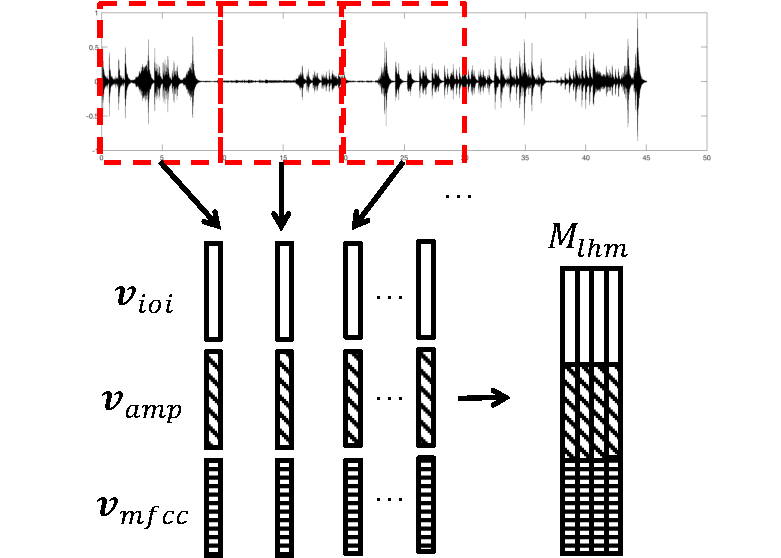
\includegraphics[width = 8 cm]{./figs/hist_mat.pdf}
\caption{Illustration of the construction process of local histogram matrix; $\mathbf{v}_{ioi}$ is the IOI histogram vector, $\mathbf{v}_{amp}$ is the amplitude histogram vector, $\mathbf{v}_{mfcc}$ is the averaged MFCCs vector, and $M_{lhm}$ is the local histogram matrix.}
\label{fig:hist_mat}
\end{figure}

\subsection{Feature Learning}\label{subsec:feat_learn}
% sparse coding
The feature learning algorithm used in this paper is Sparse Coding, which can be expressed as Eq.~\ref{eq:lasso}
\begin{equation}\label{eq:lasso}
\hat{\alpha} = \mathop{\mathrm{argmin}}_\alpha \frac{1}{2} \| X - D\alpha \|_{2}^{2} + \lambda \| \alpha \|_{1}
\end{equation}

in which the $X \in R^{ m \times n}$ is the matrix  such as $M_{stft}$ or $M_{lhm}$; $D$ is the $m \times k$ dictionary matrix, $\alpha$ is the $k \times n$ sparse matrix, $\lambda$ is the sparsity coefficient, $n$ is the number of local segments, and $k$ is the user-defined dictionary size. 

This $l1$ regularized Least Absolute Shrinkage and Selection Operator (LASSO) problem can be solved by Least Angle Regression (LARS)\cite{Efron2004} algorithm efficiently, in which the dictionary $D$ and the sparse matrix $\alpha$ can be learned by iteratively minimizing the reconstruction loss. Finally, the resulting dictionary $D$ can be considered as the feature extractor, where the corresponding sparse representation $\alpha$ can be used to compute the features. 

To compute the final feature vector that represents each audio recording, our system first learns an universal dictionary $D_{all}$ from the entire dataset. This can be done by concatenating the $M_{stft}$ or $M_{lhm}$ across all the training files, and solve the LASSO optimization problem on the concatenated matrix $X_{all}$. Next, the $\alpha_{individual}$ is estimated from each recording by substituting the $X$ in Eq.~\ref{eq:lasso} with the input representation of an individual file $X_{individual}$ while keeping the $D = D_{all}$ fixed throughout the optimization process. The resulting $\alpha_{individual}$ is a $k \times n$ sparse matrix. Finally, $\alpha_{individual}$ is aggregated using mean and standard deviation across $n$ segments, producing a feature vector $\mathbf{\alpha_{final}} = [mean(\alpha_{individual}); std(\alpha_{individual})]$ with a dimensionality of $d_{final} = 2 \times k$.  

In our experiment, the Matlab implementation of the SC from the open source library SPAMS\footnote{http://spams-devel.gforge.inria.fr Last accessed: 2017/04/26}\cite{Mairal2009a} is used. For parameterization, $k = \{32, 64, 128\}$ has been tested, and the sparsity coefficient $\lambda = \frac{1}{\sqrt{block size}}$ is applied. 

\subsection{Regression Model}
% SVR training and outlier removal
The regression model used in this paper is the Support Vector Regression (SVR) with a linear kernel. The Matlab implementation of this algorithm from open source library, libsvm \cite{Chang2011}, is used with default settings. Due to the limited size of sample pool (See Sect.~\ref{subsec:dataset} for more details), a Leave One Out (LOO) cross-validation scheme is applied to our evaluation process. The main idea of LOO is to sequential select one sample from the pool as testing data and use the rest of the pool as training data until all the samples have been tested. Additionally, an outlier removal process is implemented by iteratively removing the sample with the largest residual between the prediction and the actual label until 5\% of the entire data is eliminated. This process potentially helps the regressor to better capture the underlying patterns of the data.  

\section{Experiments}\label{sec:experiments}
\subsection{Dataset}\label{subsec:dataset}

% ===== OVERVIEW OF FBA DATASET
\begin{table}[]
\centering
\begin{tabular}{ccccc}
\hline
\multirow{2}{*}{\textbf{Year}}       & \multicolumn{3}{c}{\textbf{Group}}                                                                                                                                                                                       & \multirow{2}{*}{\textbf{Total}}      \\ \cline{2-4}
                                     & \textbf{\begin{tabular}[c]{@{}c@{}}Middle\\ School\end{tabular}}       & \textbf{\begin{tabular}[c]{@{}c@{}}Concert\\ Band\end{tabular}}       & \textbf{\begin{tabular}[c]{@{}c@{}}Symphonic\\ Band\end{tabular}}       &                                      \\ \hline
2013                                 & 1099                                                                   & 984                                                                   & 1200                                                                    & 3283                                 \\
2014                                 & 1133                                                                   & 1052                                                                  & 1368                                                                    & 3553                                 \\
2015                                 & 1106                                                                   & 1102                                                                  & 1378                                                                    & 3586                                 \\ \hline
\multicolumn{5}{c}{\textbf{List of all instruments}}                                                                                                                                                                                                                                                   \\ \hline
\multicolumn{5}{c}{\begin{tabular}[c]{@{}c@{}}Alto Sax, Baritone Sax, Bass Clarinet, \\ Bass Trombone, Bassoon, Bb Clarinet, \\ Bb Contrabass Clarinet, Eb Clarinet, English Horn, \\ Euphonium, Flute, French Horn, Oboe, \\ Percussion, Piccolo, Tenor Sax,\\  Trombone, Trumpet, Tuba\end{tabular}} \\ \hline
\end{tabular}
\caption{An overview of numbers of student recordings in FBA dataset from 2013 to 2015}
\label{tab:fba_all}
\end{table}

% information about the overall dataset
The dataset used for this study is provided by the Florida Bandmasters Association (FBA). This dataset contains audio recordings from the Florida all-state auditions of three groups of students: middle school (7th and 8th graders), concert band (9th and 10th graders), and symphonic band (11th and 12th graders) for three consecutive years (2013 to 2015). A total number of 19 types of instruments are included in the auditions. As a result, this dataset can be split into different subsets of recordings by their year, group, and instrument (e.g., 2013, middle school, clarinet). Each subset contains up to 180 recordings of student performances.  

In each recording, a student is required to perform several exercises, such as technical etude, lyrical etude, chormatic scale, 12 major scales, and sight-reading. Each exercise is graded by the judges using assessment categories such as musicality, note accuracy, rhythmic accuracy, tone quality, artistry, and articulation. The maximum score of these categories vary from 5 to 40. In our experiments, all of the ratings are normalized to a range between 0 and 1 by dividing the score with the maximum allowed value of the corresponding category. An overview of the FBA dataset is shown in Table \ref{tab:fba_all}. More information and implementations related to this paper can be found in the Github repository\footnote{http://dummy.link}.  

In this paper, the focus is on assessing percussion instrument. For percussion instruments, the audition session includes 5 different exercises, which are mallet etude, snare etude, chromatic scale (xylophone), 12 major scales (xylophone), and sight-reading (snare). To further narrow down the scope of this study, we use only the subset of middle school snare etude from all three years. This particular combination is selected for containing a comparably high number of students. As shown in Table \ref{tab:fba_snare}, a total number of 274 recordings of snare etude with an averaged duration of 51.3 seconds is available for analysis. For this particular exercise, the assessment categories include musicality (L1) and rhythmic accuracy (L2).


%===== details of snare etude recordings
\begin{table}[]
\centering
\begin{tabular}{cccc}
\hline
\multicolumn{4}{c}{\textbf{Middle school/ Percussion/ Snare Etude}}                                                                                                               \\ \hline
\textbf{Year} & \textbf{\#Students} & \textbf{\begin{tabular}[c]{@{}c@{}}Total Dur \\ (sec)\end{tabular}} & \textbf{\begin{tabular}[c]{@{}c@{}}Averaged Dur\\ (sec)\end{tabular}} \\ \hline
2013          & 98                  & 4953                                                                & 50                                                                    \\
2014          & 90                  & 4595                                                                & 51                                                                    \\
2015          & 86                  & 4608                                                                & 53                                                                    \\ \hline
\end{tabular}
\caption{Statics of the middle school snare etude from 2013 to 2015}
\label{tab:fba_snare}
\end{table}

\subsection{Experiment Setup}
This paper presents two experiments that highlight different characteristics of the proposed feature learning method in the context of assessing student snare drum performances.

% Experiment 1: feature learning from two different input representations
In Experiment 1, the effectiveness of two different input representations (See Sect.~\ref{subsec:input}) for SC is compared. The tested configurations are listed as follows:
\begin{enumerate}[(i)]
\item \textbf{SC + STFT}: Sparse coding features using STFT as input representations
\item \textbf{SC + LHM}: Sparse coding features using LHM as input representations 
\end{enumerate}
Both configurations are tested using $k = \{32, 64, 128\}$.\\

% Experiment 2: comparison between different combination of feature sets
In Experiment 2, the regression model trained on the SC learned features using the proposed LHM with $k = 32$ is compared to two different sets of features proposed by Wu et al.~\cite{Wu2016}, namely the baseline and designed features. The regression performances of the following feature combinations are tested:
\begin{enumerate}[(i)]
\item \textbf{Baseline}: the standard spectral and temporal features such as spectral centroid, spectral rolloff, spectral flux, zero-crossing rate, and 13 MFCCs (See \cite{Wu2016} for more details). $d_{baseline} = 68$
\item \textbf{Designed}: the desgined rhythmic and dynamic features derived from the IOI and amplitude histograms (See \cite{Wu2016} for more details). $d_{designed} = 18$
\item \textbf{SC (Proposed)}: the SC learned features as described in Sect.~\ref{subsec:feat_learn}
\item \textbf{Baseline + Designed}: a combined feature set consists of both baseline and designed features 
\item \textbf{SC + Baseline}:  a combined feature set consists of both SC and baseline features 
\item \textbf{SC + Designed}:  a combined feature set consists of both SC and designed features 
\item \textbf{All}: a combination of all three sets of features
\end{enumerate}

\subsection{Metrics}
The performance of the models is investigated using the following standard statistical metrics: the Pearson correlation coefficient $r$ and the coefficient of determination (i.e., $R^{2}$). These metrics are commonly used to evaluate the strength of the relationship between the regression predictions and ground truth. Details of the mathematical formulations can be found in \cite{McClave2003}. 

\subsection{Experiment Results}
\begin{table}[]
\centering
\begin{tabular}{cccccc}
\hline
\multicolumn{2}{c}{Input Representation}                                             & \multicolumn{2}{c}{STFT} & \multicolumn{2}{c}{LHM}       \\ \hline
\begin{tabular}[c]{@{}c@{}}Dictionary \\ Size\end{tabular} & Metrics                 & L1         & L2          & L1            & L2            \\ \hline
\multirow{2}{*}{k = 32}                                    & r                       & 0.34       & 0.19        & 0.65          & \textbf{0.57} \\
                                                           & $R^{2}$ & 0.08       & -0.02       & 0.41          & \textbf{0.29} \\ \hline
\multirow{2}{*}{k = 64}                                    & r                       & 0.41       & 0.26        & \textbf{0.70} & 0.50          \\
                                                           & $R^{2}$ & 0.11       & -0.00       & \textbf{0.45} & 0.06          \\ \hline
\multirow{2}{*}{k = 128}                                   & r                       & 0.41       & 0.28        & 0.33          & 0.34          \\
                                                           & $R^{2}$ & 0.08       & -0.07       & -0.08         & -0.78         \\ \hline
\end{tabular}
\caption{Evaluation results for Experiment 1: L1 represents musicality, and L2 represents rhythmic accuracy}
\label{tab:exp1}
\end{table}

% LHM outperform STFT overall. STFT can't capture the temporal information 
% when k is large, both perform poorly (274 samples, when k = 128, the feature has a d = 2*k = 256) which could bring a lot of noise
% when k = 32, the improvement is the largest. 
In this section, the evaluation results of Experiment 1 and Experiment 2 are presented and discussed. It should be noted that since all of the correlation results are significant ($p << 0.05$), their p-values are not reported.  

The evaluation results of Experiment 1 is shown in Table\ref{tab:exp1}. The following trends can be observed: first, LHM almost outperform STFT in every case. This result clearly indicates that LHM is a more effective input representation for SC compared with STFT. One possible explanation for this discrepancy could originate from the their capabilities of capturing the temporal information. Since STFT only represents the spectral shapes at various instances, it does not encapsulate any temporal dependencies between meaningful audio events such as consecutive drums hits. These temporal information, while being likely to reside in the sparse matrix $\alpha$, will be destroyed after the feature aggregation. This absence of temporal information poses a problem for SC to learn higher level music concept such as rhythm. LHM, on the other hand, captures the temporal dependencies between the audio events with the IOI histograms. This ensures the rhythmic information to be translated into the SC dictionary and reflect on the final features, leading towards a better performance. Second, when the dictionary size $k = 128$, both STFT and LHM perform poorly. The reason behind this degradation for both representations might be due to the limited size of the sample pool. When $k = 128$, the resulting feature dimensionality, as described in Sect.~\ref{subsec:feat_learn}, would be $k \times 2 = 256$. This will result in a feature matrix of $274 (students) \times 256 (features)$, and the model could suffer from the curse of dimensionality. Potential solution to this problem is through dimensionality reduction methods such as Principle Component Analysis (PCA) or feature selections, however, it is currently out of the scope of this study. Third, when $k = 32$, the LHM has the largest improvement over STFT in both L1 and L2. This result might suggest a relationship between the best performing $k$ and the number of samples in the dataset, but this would require further investigations. 

% Experiment 2

\begin{figure*}
\centering
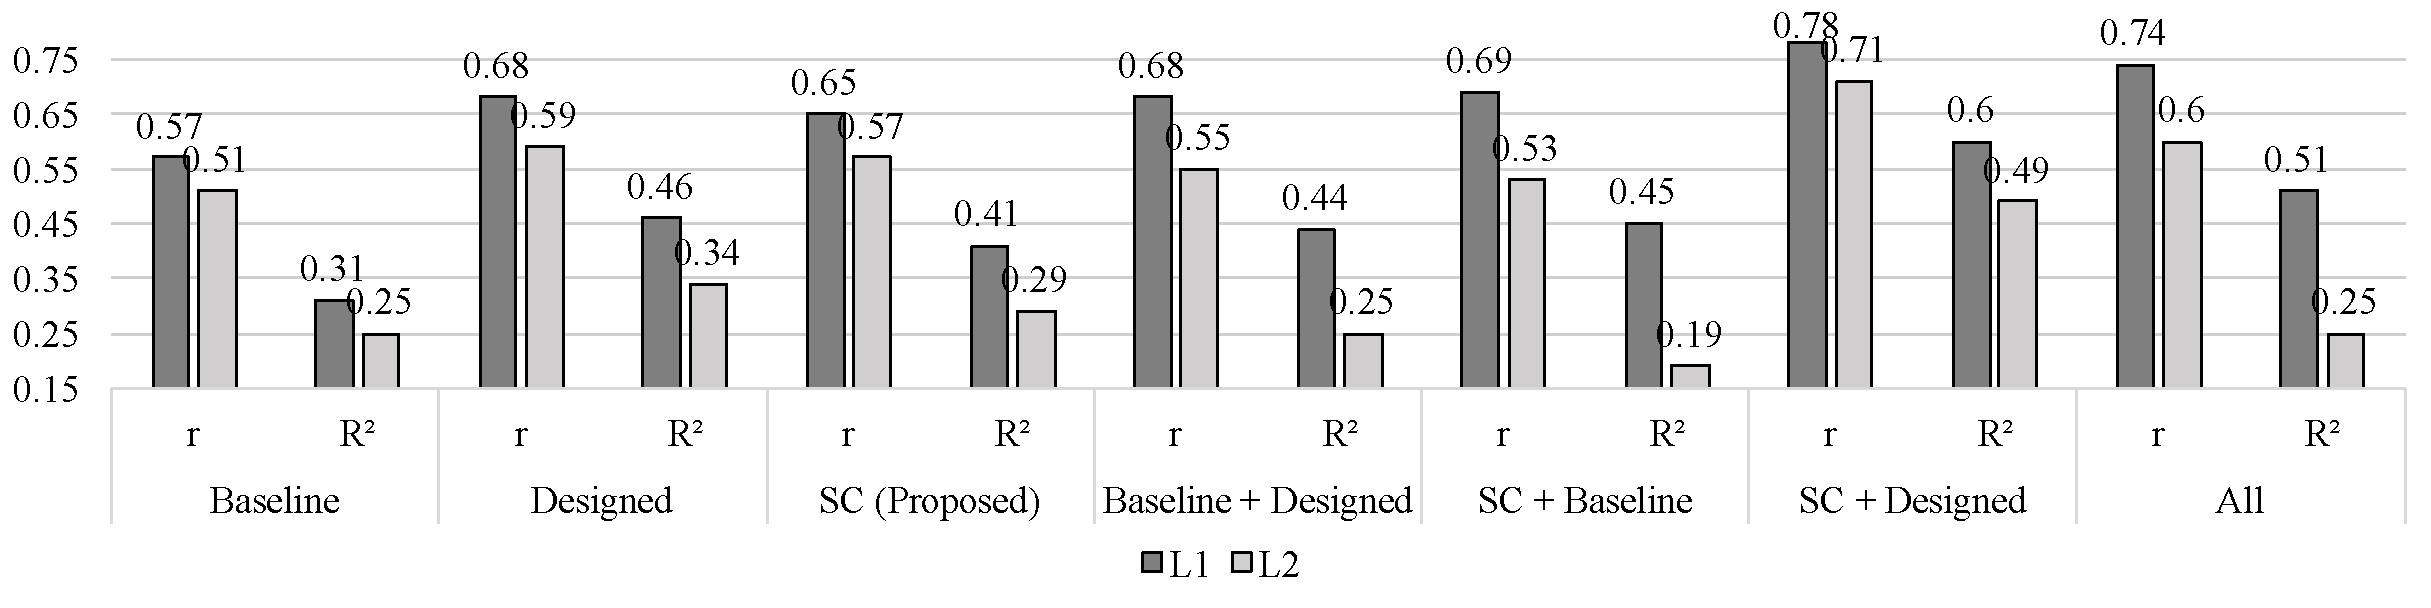
\includegraphics[width = 17.2 cm]{./figs/exp2.pdf}
\caption{Evaluation results for Experiment 2}
\label{fig:exp2}
\end{figure*}
% Short summary

% first thing to 
The evaluation results of Experiment 2 is shown in Fig.~\ref{fig:exp2}. The first thing to notice is that, the proposed SC features achieve comparable performances with the designed features, and they both outperform the baseline features. Since the baseline features are only instantaneous features that are not optimized to the task, their inferior performances are conceivable. The fact that SC features perform similarly to the designed features is encouraging, suggesting the possibility of deriving viable features with minimum effort in feature crafting. Next, when combined with baseline features, both designed and SC features exhibit almost no improvements. This issue could be similar to the situation when having a large $k$ as discussed in Experiment 1, for baseline features might facilitate the curse of dimensionality by introducing too many features in the current size of sample pool. Among all the tests in Experiment 2, the highest performance is achieved with the combination of designed and SC features. The result implies the effectiveness of SC features in bringing non-redundant information to the designed features and is generally promising. This demonstrates the potential of using feature learning method to further optimize the human designed features by exploring the internal structure of the data.   

Another commonality that can be summarized from both Experiment 1 and Experiment 2 is the superior performances of modeling L1 over L2. As discussed in \cite{Wu2016}, musicality is an abstract but holistic measure of the performance, and it is therefore more likely to be consistently graded. 

% conclude from both experiments: musicality is easier to model
\section{Conclusion}\label{sec:conclusion}
% we show the importance of input representation prior to feature learning. The experiment results show that a good intermediate feature representation is important
This paper presents an unsupervised feature learning approach to derive features for assessing percussive instrument performances. Specifically, we propose to use LHM as the input representation to SC that will better capture the temporal information and lead to better results. The advantage of this work include: first, it provides insights to the selection of input representation for SC in the context of snare drum performance assessment. Second, the proposed SC features achieve comparable results with the designed features, demonstrate the viability of deriving competitive features with minimum effort in feature designing. Finally, combining the designed features with the SC features, the highest performance can be achieved. This result suggests that SC features might be able to provide complementary information to the features designed with domain knowledge, further optimizing the performance of a given task. 

The possible future directions of this work include: 
\begin{inparaenum}[(i)]
    \item   Evaluate and compare the efficiency of different feature learning algorithms. Methods such as DBN\cite{Hamel2010} and denoising autoencoders \cite{Vincent2008} may provide new insights into the finding of the best feature learning strategy for automatic performance assessment.
    \item   Adapt the proposed method to other types of instruments such as Brass or Woodwind instruments. The evaluation results on the melodic instruments should lead to the refinement of the proposed feature learning scheme. 
    \item   More data. To further investigate the robustness and generality of this approach, more data is needed. Additionally, the increase in sample pool can also help the investigation into the relationship between dictionary size $k$ and the number of samples. This might lead to a better strategy for selecting the best performing $k$. 
\end{inparaenum}

% For bibtex users:
\bibliography{cw_ismir2017_fba}

\end{document}
